\documentclass[border=3pt]{standalone}
\usepackage{tikz}
\usetikzlibrary{positioning, arrows.meta, calc, fit, backgrounds}
\usepackage{amsmath}
\begin{document}
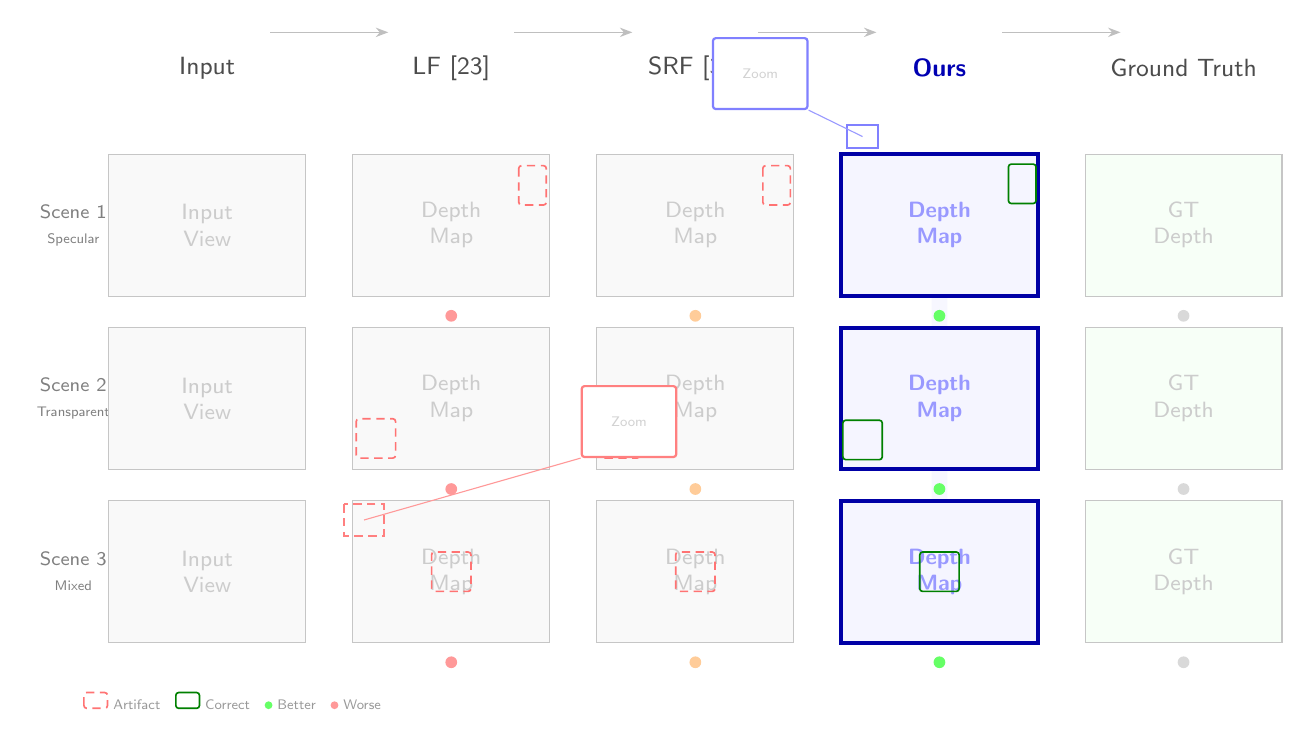
\begin{tikzpicture}[
    img/.style={draw=gray!45, minimum width=2.5cm, minimum height=1.8cm,
                inner sep=0pt, align=center, fill=gray!5,
                font=\sffamily\footnotesize, text=gray!40},
    ours/.style={draw=blue!65!black, minimum width=2.5cm, minimum height=1.8cm,
                 inner sep=0pt, align=center, fill=blue!4,
                 font=\sffamily\footnotesize\bfseries, text=blue!40,
                 line width=1.5pt},
    gt/.style={draw=gray!45, minimum width=2.5cm, minimum height=1.8cm,
               inner sep=0pt, align=center, fill=green!3,
               font=\sffamily\footnotesize, text=gray!40},
    hdr/.style={font=\sffamily\small, text=black!70},
    sclbl/.style={font=\sffamily\scriptsize, text=black!50, align=center},
    farr/.style={-{Stealth[length=4.5pt]}, semithick, color=black!25},
    emark/.style={draw=red!55, densely dashed, line width=0.6pt, rounded corners=1pt},
    gmark/.style={draw=green!50!black, line width=0.6pt, rounded corners=1pt},
]

% Positions
\pgfmathsetmacro{\xA}{0}
\pgfmathsetmacro{\xB}{3.1}
\pgfmathsetmacro{\xC}{6.2}
\pgfmathsetmacro{\xD}{9.3}
\pgfmathsetmacro{\xE}{12.4}
\pgfmathsetmacro{\yH}{0.6}
\pgfmathsetmacro{\yI}{-1.4}
\pgfmathsetmacro{\yII}{-3.6}
\pgfmathsetmacro{\yIII}{-5.8}

% ===== HEADERS =====
\node[hdr] at (\xA, \yH) {Input};
\node[hdr] at (\xB, \yH) {LF~[23]};
\node[hdr] at (\xC, \yH) {SRF~[31]};
\node[hdr, text=blue!70!black] at (\xD, \yH) {\textbf{Ours}};
\node[hdr] at (\xE, \yH) {Ground Truth};

% Flow arrows
\draw[farr] (0.8, 1.05) -- (2.3, 1.05);
\draw[farr] (3.9, 1.05) -- (5.4, 1.05);
\draw[farr] (7.0, 1.05) -- (8.5, 1.05);
\draw[farr] (10.1, 1.05) -- (11.6, 1.05);

% ===== BACKGROUND HIGHLIGHT FOR OURS =====
\begin{scope}[on background layer]
    \fill[blue!3, rounded corners=3pt]
        (\xD-0.1, -0.95) rectangle (\xD+0.1, -6.35);
\end{scope}

% ===== ROW 1: Specular =====
\node[sclbl] at (-1.7, \yI) {Scene 1\\[1pt]{\tiny Specular}};
\node[img] (R1A) at (\xA, \yI) {Input\\View};
\node[img] (R1B) at (\xB, \yI) {Depth\\Map};
\node[img] (R1C) at (\xC, \yI) {Depth\\Map};
\node[ours] (R1D) at (\xD, \yI) {Depth\\Map};
\node[gt] (R1E) at (\xE, \yI) {GT\\Depth};

% ===== ROW 2: Transparent =====
\node[sclbl] at (-1.7, \yII) {Scene 2\\[1pt]{\tiny Transparent}};
\node[img] (R2A) at (\xA, \yII) {Input\\View};
\node[img] (R2B) at (\xB, \yII) {Depth\\Map};
\node[img] (R2C) at (\xC, \yII) {Depth\\Map};
\node[ours] (R2D) at (\xD, \yII) {Depth\\Map};
\node[gt] (R2E) at (\xE, \yII) {GT\\Depth};

% ===== ROW 3: Mixed =====
\node[sclbl] at (-1.7, \yIII) {Scene 3\\[1pt]{\tiny Mixed}};
\node[img] (R3A) at (\xA, \yIII) {Input\\View};
\node[img] (R3B) at (\xB, \yIII) {Depth\\Map};
\node[img] (R3C) at (\xC, \yIII) {Depth\\Map};
\node[ours] (R3D) at (\xD, \yIII) {Depth\\Map};
\node[gt] (R3E) at (\xE, \yIII) {GT\\Depth};

% ===== ERROR/GOOD REGION MARKERS =====
% Scene 1: error on upper-right of B, C; good on D
\draw[emark] ([shift={(-0.4,-0.15)}]R1B.north east) rectangle ([shift={(-0.05,-0.65)}]R1B.north east);
\draw[emark] ([shift={(-0.4,-0.15)}]R1C.north east) rectangle ([shift={(-0.05,-0.65)}]R1C.north east);
\draw[gmark] ([shift={(-0.4,-0.15)}]R1D.north east) rectangle ([shift={(-0.05,-0.65)}]R1D.north east);

% Scene 2: error on lower-left of B, C; good on D
\draw[emark] ([shift={(0.05,0.15)}]R2B.south west) rectangle ([shift={(0.55,0.65)}]R2B.south west);
\draw[emark] ([shift={(0.05,0.15)}]R2C.south west) rectangle ([shift={(0.55,0.65)}]R2C.south west);
\draw[gmark] ([shift={(0.05,0.15)}]R2D.south west) rectangle ([shift={(0.55,0.65)}]R2D.south west);

% Scene 3: error on center of B, C; good on D
\draw[emark] ([shift={(-0.25,-0.25)}]R3B.center) rectangle ([shift={(0.25,0.25)}]R3B.center);
\draw[emark] ([shift={(-0.25,-0.25)}]R3C.center) rectangle ([shift={(0.25,0.25)}]R3C.center);
\draw[gmark] ([shift={(-0.25,-0.25)}]R3D.center) rectangle ([shift={(0.25,0.25)}]R3D.center);

% ===== ZOOM PATCHES =====
% Scene 1: zoom region on R1D
\draw[blue!50, line width=0.7pt] ([shift={(0.1,0.05)}]R1D.north west) rectangle ([shift={(0.5,0.35)}]R1D.north west);

% Zoom inset for scene 1
\node[draw=blue!50, fill=white, minimum width=1.2cm, minimum height=0.9cm,
      font=\sffamily\tiny, text=gray!35, rounded corners=1pt,
      line width=0.8pt] (zoom1) at ([shift={(-1.0,1.0)}]R1D.north west) {Zoom};
\draw[blue!40, thin] ([shift={(0.3,0.2)}]R1D.north west) -- (zoom1.south east);

% Scene 3: zoom region on R3B
\draw[red!50, densely dashed, line width=0.7pt] ([shift={(-0.1,-0.05)}]R3B.north west) rectangle ([shift={(0.4,-0.45)}]R3B.north west);

% Zoom inset for scene 3
\node[draw=red!50, fill=white, minimum width=1.2cm, minimum height=0.9cm,
      font=\sffamily\tiny, text=gray!35, rounded corners=1pt,
      line width=0.8pt] (zoom3) at ([shift={(1.0,1.0)}]R3B.north east) {Zoom};
\draw[red!40, thin] ([shift={(0.15,-0.25)}]R3B.north west) -- (zoom3.south west);

% ===== QUALITY INDICATORS (small colored dots) =====
\foreach \yy in {\yI, \yII, \yIII} {
    \node[circle, fill=red!40, inner sep=1.5pt] at (\xB, \yy-1.15) {};
    \node[circle, fill=orange!40, inner sep=1.5pt] at (\xC, \yy-1.15) {};
    \node[circle, fill=green!60, inner sep=1.5pt] at (\xD, \yy-1.15) {};
    \node[circle, fill=gray!30, inner sep=1.5pt] at (\xE, \yy-1.15) {};
}

% ===== LEGEND =====
\node[font=\sffamily\tiny, text=black!40, anchor=north west] at (-1.7, -7.2) {%
    \tikz\draw[emark] (0,0) rectangle (0.3,0.2); Artifact\quad
    \tikz\draw[gmark] (0,0) rectangle (0.3,0.2); Correct\quad
    \tikz\node[circle, fill=green!60, inner sep=1pt]{}; Better\quad
    \tikz\node[circle, fill=red!40, inner sep=1pt]{}; Worse
};

\end{tikzpicture}
\end{document}